%!TEX root = ../../Thesis.tex

\section{Evaluation: Microbenchmarks}
\label{sec:micro}

We consider a set of micro-benchmarks inspired from real-world applications 
(\sectref{micro-benchmarks}) and evaluate the number of test iterations
required to fail an invalid assertion 
(\sectref{micro-assertion-violations}). We also measure the \textit{coverage} of
weak behaviors provided by MonkeyDB (\sectref{micro-coverage}). Each of these
applications were implemented based on their specifications described in prior
work; they all use MonkeyDB as a library, via its KV interface.  

%, also used in previous work, that are inspired
%from real-world applications:  
%Courseware~\cite{DBLP:conf/esop/NairP020}, Shopping
%cart~\cite{DBLP:conf/pldi/Sivaramakrishnan15} and Twitter~\cite{twissandra}, and
%also a concurrent stack data-structure \cite{DBLP:conf/cav/NagarMJ20}.
%We describe these applications in \sectref{micro-benchmarks}. We
%perform two kinds of experiments. We evaluate the number of test iterations
%required to fail an invalid assertion 
%(\sectref{micro-assertion-violations}) and we also measure the \textit{coverage} of
%weak behaviors provided by MonkeyDB (\sectref{micro-coverage}). Each of these
%use MonkeyDB as a library, via its KV interface.  

\subsection{Applications}
\label{sec:micro-benchmarks}

\paragraph{Twitter \cite{twissandra}}
This is based on a social-networking application that allows users to create a new account, follow,
unfollow, tweet, browse the newsfeed (tweets from users you follow)
and the timeline of any particular user. 
%More formally, $U$ is the set of all users,
%each user has a set of tweets $U.T$, a set of following user $U.FW$ and set of
%followers $U.FR$. 
\figref{twitter-algo} shows the pseudo code for two operations. 
%In \texttt{NewsFeed} and \texttt{Timeline} operations, tweets are
%always returned sorted to the user, by time.

A user can access twitter from multiple clients (sessions), which could lead to
unexpected behavior under weak consistency models. 
Consider the following scenario with two users, $A$ and $B$ where user $A$ is accessing twitter from two
different sessions, $S_1$ and $S_2$. User $A$ views the timeline of user $B$
from one session (\texttt{$S_1$:Timeline($B$)}) and decides to follow $B$
through another session (\texttt{$S_2$:Follow($A$, $B$)}). Now when user $A$
visits their timeline or newsfeed (\texttt{$S_2$:NewsFeed($A$)}), they expect to
see all the tweets of $B$ that were visible via \texttt{Timeline} in session $S_1$. But
under weak consistency models, this does not always hold true and there could
be missing tweets. 

\begin{figure}
\centering
  \begin{tabular}{@{\hspace{0ex}}l@{\hspace{-1ex}}l}
	\begin{minipage}{4cm}
		\begin{lstlisting}[basicstyle=\ttfamily\footnotesize,escapeinside={(*}{*)},language=MyLang]
			
// Get user's tweets
Timeline(user u) {
  Begin()
  key = "tweets:" + u.id
  T = read(key) 
  Commit()
  return sortByTime(T)
}
		\end{lstlisting}
	\end{minipage}
  &
	%\hspace{-5mm}
	\begin{minipage}{4.3cm}
		\begin{lstlisting}[xleftmargin=3mm,basicstyle=\ttfamily\footnotesize,escapeinside={(*}{*)},language=MyLang]
// Get following users' tweets
NewsFeed(user u) {
  Begin()
  FW = read("following:"+ u.id)
  NF = {}
  foreach v (*$\in$*) FW:
    T = read("tweets:"+ v.id)
    NF = NF (*$\cup$*) T
  Commit()
  return sortByTime(NF)
}
		\end{lstlisting}
	\end{minipage}
\end{tabular}
\vspace{-5ex}
	\caption{Example operations of the Twitter app}
	\label{fig:twitter-algo}
\end{figure}

\vspace{-2mm}
\paragraph{Shopping Cart \cite{DBLP:conf/pldi/Sivaramakrishnan15}}
This application allows a user to add,
remove and change quantity of items from different sessions. It also allows the
user to view all items present in the shopping cart. The pseudo code and
an unexpected behavior under weak consistency models were discussed in
\sectref{app:intro}, \figref{motiv}.

\vspace{-2mm}	
\paragraph{Courseware \cite{DBLP:conf/esop/NairP020}}
This is an application for managing students and courses, allowing students
to register, de-register and enroll for courses. Courses can also be created 
or deleted. Courseware maintains the current status of
students (registered, de-registered), courses (active, deleted) as well as
enrollments.
%$S.P$ and $S.N$ are
%the set of registered students and de-registered students respectively.
%Similarly, $C.P$ and $C.N$ are for created and deleted courses. 
Enrollment can contain only registered students and active courses, subject to the capacity
of the course.
%, i.e., $E = \{(u, v) | u \in S.P, v \in C.P\}$ such that $ \forall
%v \in C.P : |\{(u, v) \in E\}| \leq capacity(v)$.  
%\figref{courseware-algo} shows an implementation of the \texttt{Enroll} operation.

Under weak isolation, it is possible that two different students, when trying to
enroll concurrently, will both succeed even though only one spot was left in the
course. Another example that breaks the application is when a student is trying
to register for a course that is being concurrently removed: once the course is
removed, no student should be seen as enrolled in that course.


%\begin{figure}
%\begin{lstlisting}[mathescape=true,language=MyLang]
%Enroll(student s, course c) {
%    Begin()
%    S = read("students") // registered students
%    C = read("courses")  // active courses
%    if (s $\notin$ S || c $\notin$ C)
%      throw InvalidEnrollment;
%    E = read("enrollments")
%    if |{u: (u, c) $\in$ E}| == capacity(c)
%      throw CourseFull;
%    E = E $\cup$ {(s, c)}
%    write("enrollments", E)
%    Commit()
%}
%\end{lstlisting}
%\caption{Courseware implementation of {\tt Enroll}}
%\label{Fi:courseware-algo}
%\end{figure}

\vspace{-2mm}
\paragraph{Treiber Stack \cite{DBLP:conf/cav/NagarMJ20}}
Treiber stack is a concurrent stack data structure that uses 
compare-and-swap (CAS) instructions instead of locks for synchronization. This
algorithm was ported to operate on a kv-store in prior work \cite{DBLP:conf/cav/NagarMJ20}
and we use that implementation. Essentially, the stack contents are placed in
a kv-store, instead of using an in-memory linked data structure.
Each row in the store contains a pair consisting of the stack element and the key of the next
row down in the stack. A designated key ``{\tt head}'' stores the key of the
top of the stack. CAS is implemented as a transaction, but the 
\texttt{pop} and \texttt{push} operations do not use transactions, i.e., each
read/write/CAS is its own transaction.
%The pseudo-code is shown in \figref{stack-algo}. 
%KV stores do not provide a CAS operation, so we implement it at the application level
%using a lock-protected section of a {\tt read} and (if equal) a {\tt write}.
%We determine id of the new node based on
%the current size of the kv-store.


%\begin{figure}
%	\begin{minipage}{4.2cm}
%		\begin{lstlisting}[xleftmargin=4mm,basicstyle=\ttfamily\footnotesize,escapeinside={(*}{*)},language=MyLang]
%Push(v) {
% n = {value: v, next: null};
% while (true) {
%  top = read("head");
%  n.next = top;
%  if (CAS("head", top, n))
%   break;
% }
%}
%		\end{lstlisting}
%	\end{minipage}
%	\begin{minipage}{1mm}
%		||
%	\end{minipage}
%	\hspace{-5mm}
%	\begin{minipage}{4.2cm}
%		\begin{lstlisting}[xleftmargin=5mm,basicstyle=\ttfamily\footnotesize,escapeinside={(*}{*)},language=MyLang]
%Pop() {
% while (true) {
%  top = read("head");
%  if (top == null)
%   return EMPTY;
%  v = top.value;
%  n = top.next;
%  if (CAS("head", top, n))
%   return v;
% }
%}
%		\end{lstlisting}
%	\end{minipage}
%  \caption{Treiber stack implementation. \akash{Might be useful to show the CAS
%  implementation, key generation, etc., but in the appendix.}}
%	\label{Fi:stack-algo}
%\end{figure}

When two different clients try to \texttt{pop} from the stack concurrently, 
under serializability, each \texttt{pop} would return a unique value, assuming that each pushed value is
unique. However, under causal consistency, concurrent \texttt{pop}s can return the same
value.

	

\subsection{Assertion Checking}
\label{sec:micro-assertion-violations}

We ran the above applications with MonkeyDB to find out if assertions, capturing
unexpected behavior, were violated under causal consistency. Table
\ref{tab:assert} summarizes the results. For each application, 
we used 3 client threads and 3 operations per thread. 
We ran each test with MonkeyDB for a total of 10,000 times; we refer to a run as
an iteration. We  report the average number of iterations (Iters) 
before an assertion failed, and the corresponding time taken 
(sec). All the assertions were violated within 58 iterations, in half a second
or less. In contrast, running with an actual database almost never
produces an assertion violation.

\begin{table}[h]
  \centering
	\footnotesize
	\begin{tabular}{|l|l|c|c|}
		
		\hline
		
    \textbf{Application} & \textbf{Assertion}   & \multicolumn{2}{c|}{\textbf{Avg. time to fail}}     \\ 
                         &                      & \textbf{(Iters)} & \textbf{(sec)} \\ \hline
		
    Stack                & Element popped more than once  & 3.7  & 0.02 \\ \hline
		
    Courseware           & Course registration overflow & 10.6 & 0.09  \\ \hline
		
    Courseware           & Removed course registration & 57.5 & 0.52   \\ \hline
		
    Shopping            & Item reappears after deletion & 20.2 & 0.14  \\ \hline
		
    Twitter              & Missing tweets in feed & 6.3 & 0.03 \\ \hline
		
	\end{tabular}
	\caption{\label{tab:assert}Assertions checking results in microbenchmarks}
\end{table}

%\begin{table}[]
%	\footnotesize
%	
%	\begin{tabular}{|c|c|c|c|}
%		
%		\hline
%		
%		\textbf{ID} & \textbf{\# Failed Iters} & \textbf{First Failure} & \textbf{Avg. Time to Fail (s)} \\ \hline
%		
%		A1      &      2673                         &                    9    &     0.02                           \\ \hline
%		
%		A2          & 948                           & 17                     & 0.09                           \\ \hline
%		
%		A3          & 174                           & 18                     & 0.52                           \\ \hline
%		
%		A4          & 496                           & 36                     & 0.14                           \\ \hline
%		
%		A5          &    1595                         &   11                      &  0.03                              \\ \hline
%		
%	\end{tabular}
%	\caption{\label{tab:assert-exp}Assertion failures with MonkeyDB in 10k iterations }
%	
%\end{table}

\subsection{Coverage}
\label{sec:micro-coverage}

The previous section only checked for a particular set of assertions. As an additional measure of
test robustness, we count the number of distinct \textit{client-observable
states} generated by a test. A client-observable state, for an execution, is the vector of values returned by
read operations. For instance, a stack's state is defined by return values of 
\texttt{pop} operations; a shopping cart's state is defined by the return value
of \texttt{GetCart} and so on. 

For this experiment, we randomly generated test harnesses; each harness spawns
multiple threads that each execute a sequence of operations. In order to compute the absolute maximum
of possible states, we had to limit the size of the tests: either 2 or 3
threads, each choosing between 2 to 4 operations. 

Note that any program that concurrently executes operations against a store has
two main sources of non-determinism: the first is the interleaving of operations
(i.e., the order in which operations are submitted to the store) and second is
the choice of read-from (i.e., the value returned by the store under its
configured consistency model). MonkeyDB only controls the latter; it is up to the
application to control the former. There are many tools that systematically enumerate
interleavings (such as \textsc{Chess} \cite{DBLP:conf/pldi/MusuvathiQ08},
\textsc{Coyote} \cite{coyote-web}), but we use a simple trick
instead to avoid imposing any burden on the application: 
we included an option in MonkeyDB to deliberately add a small random
delay (sleep between $0$ to $4$ ms) before each transaction begins. This option 
was sufficient in our experiments, as we show next.

We also implemented a special setup using the \textsc{Coyote} tool \cite{coyote-web} 
to enumerate all sources of non-determinism, interleavings as well as
read-from, in order to explore the entire state space of a
test. We use this to compute the total number of states. \figref{micro_dfs}
shows the number of distinct 
states observed under different consistency models, averaged across multiple ($50$) test
harnesses. For each of serializability and causal consistency, we show the max
(as computed by \textsc{Coyote}) and versions with and without the delay option
in MonkeyDB. 

Each of these graphs show similar trends: the number of states with
causal consistency are much higher than with serializability. Thus, testing with a
store that is unable to generate weak behaviors will likely be ineffective.
Furthermore, the ``delay'' versions of MonkeyDB are able to approach the 
maximum within a few thousand attempts, implying that MonkeyDB's strategy of
per-read randomness is effective for providing coverage to the application.


\begin{figure}[!h]
	\centering
	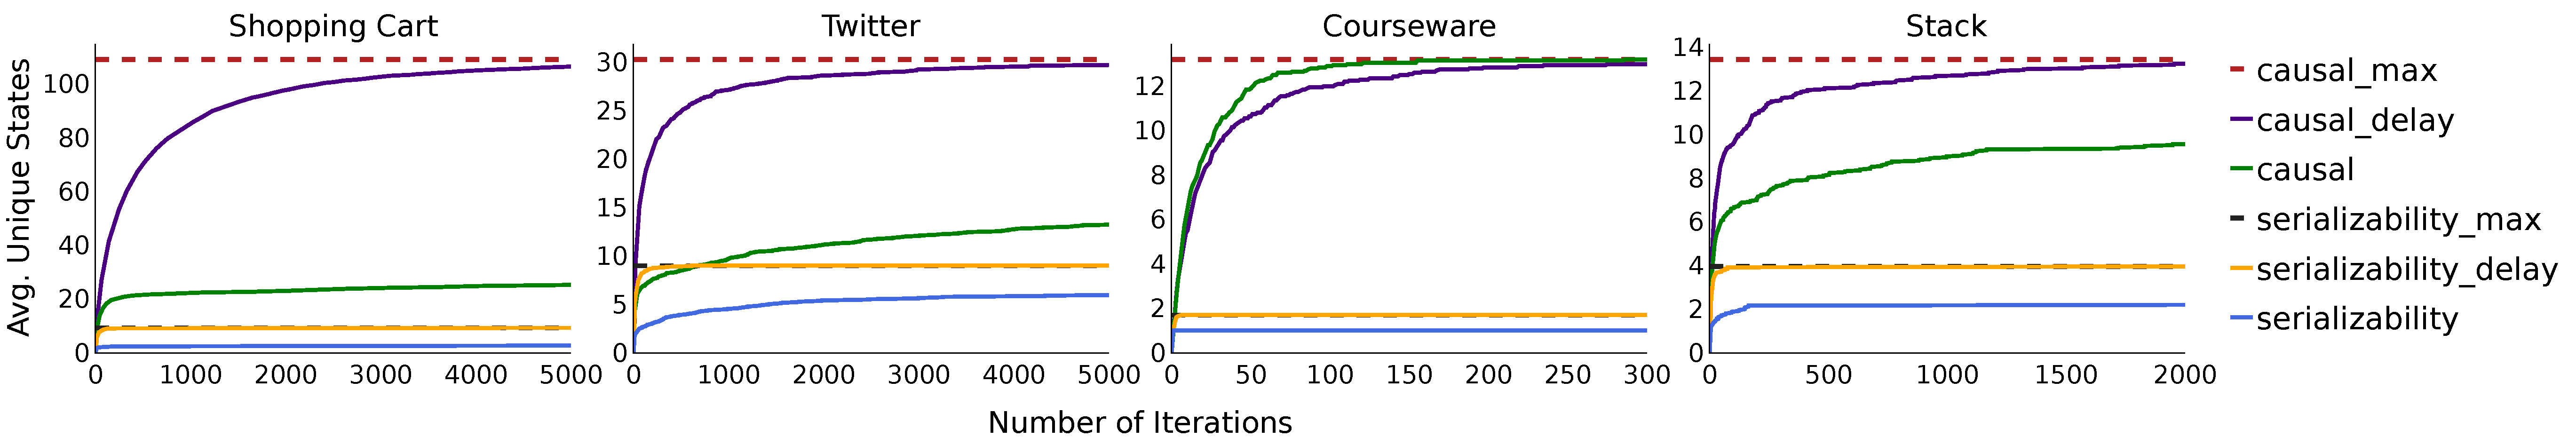
\includegraphics[width=1.0\textwidth]{Sources/sql/plots/random_avg.pdf}
	\caption{State coverage obtained with MonkeyDB for various microbenchmarks}
	\label{fig:micro_dfs}
\end{figure}

%\begin{figure}[h]
%
%	\centering
%
%	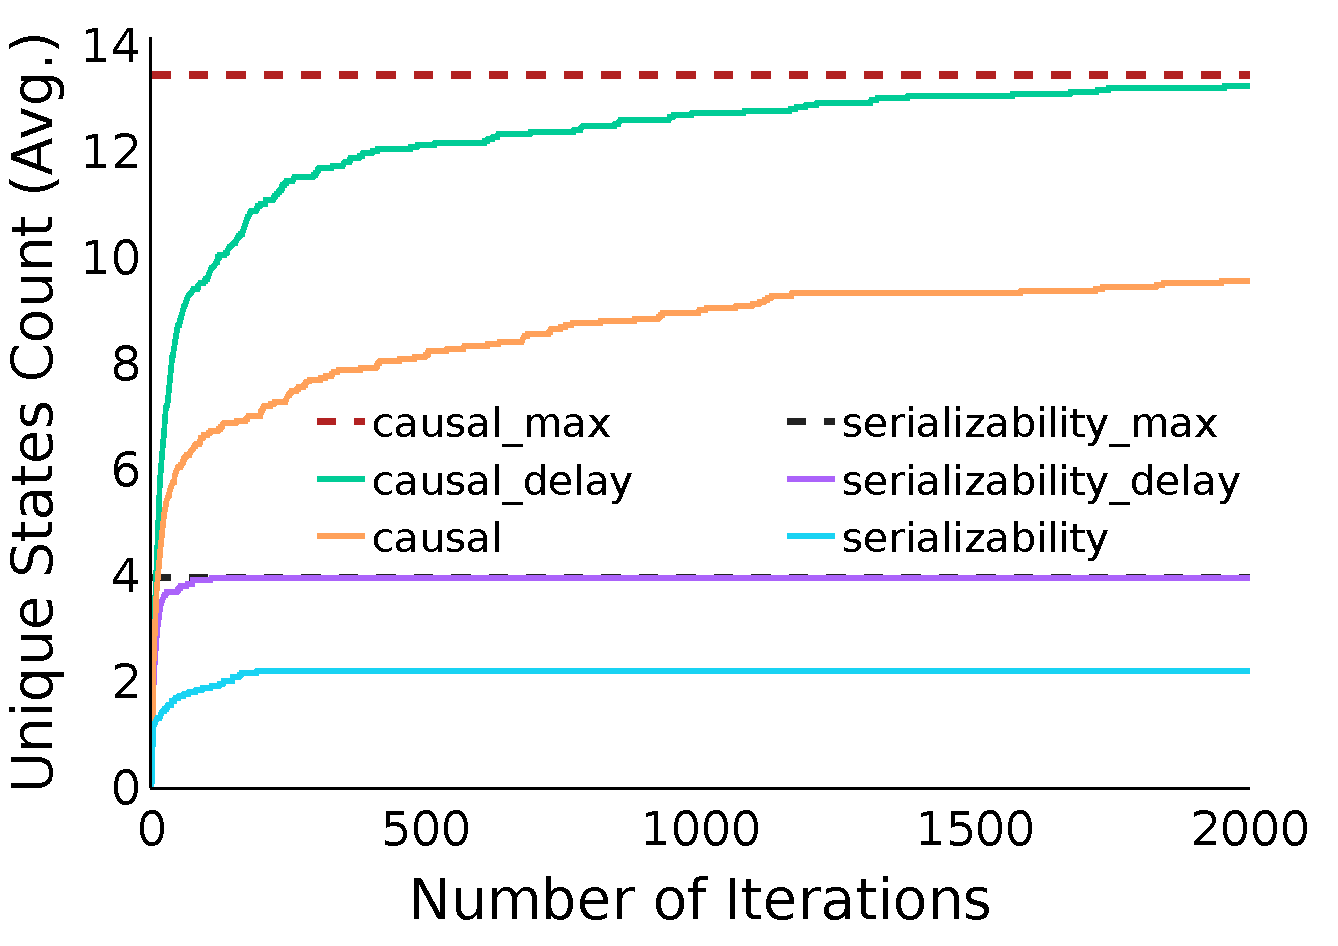
\includegraphics[width=0.4\textwidth]{plots/stack_random_avg.pdf}
%
%	\caption{Stack complete state exploration}
%
%	\label{fig:stack_dfs}
%\end{figure}
%
%
%\begin{figure}[h]
%	
%	\centering
%	
%	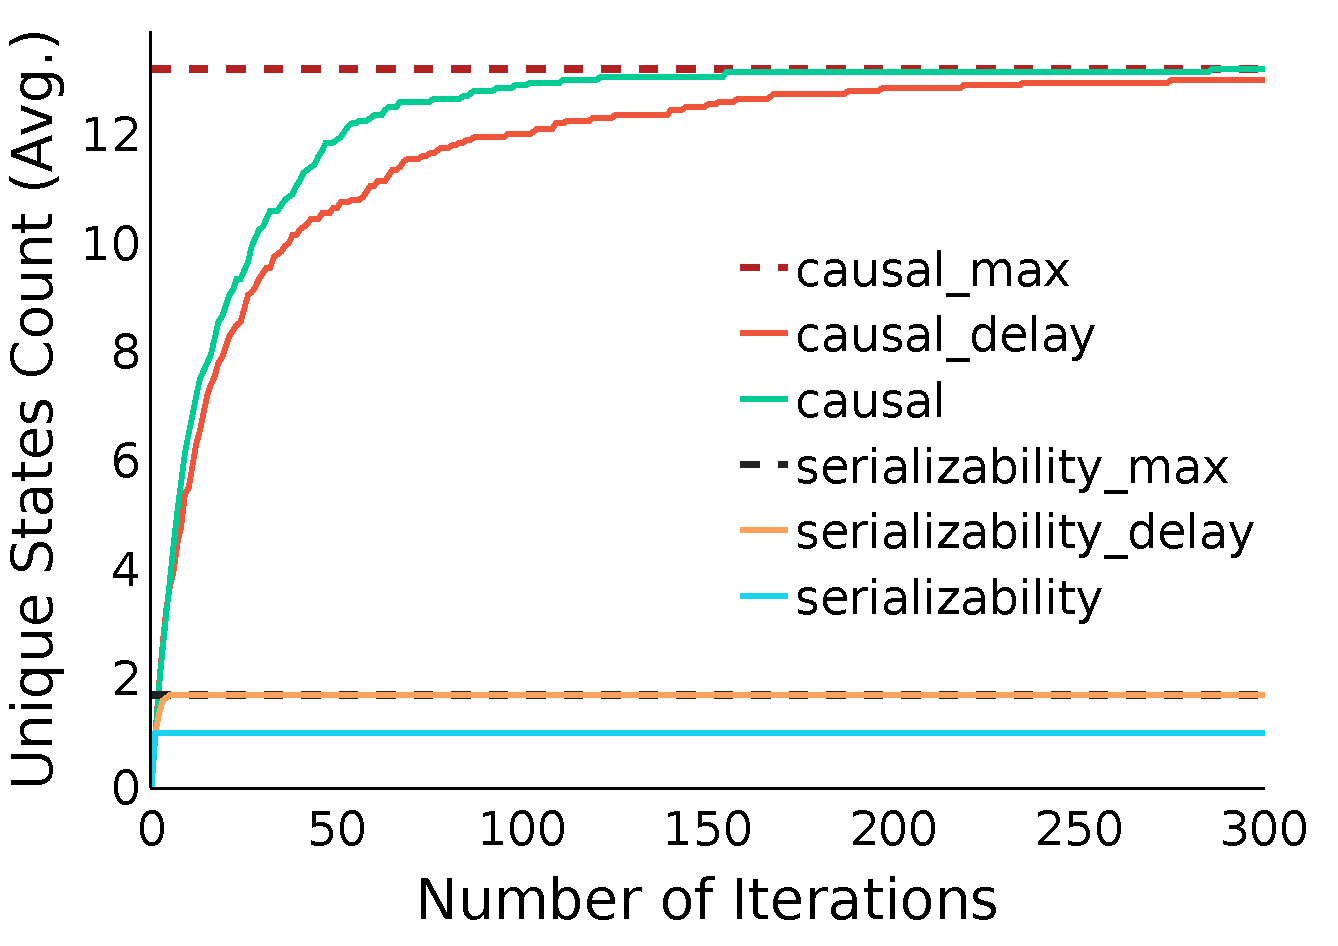
\includegraphics[width=0.4\textwidth]{plots/courseware_random_avg.pdf}
%	
%	\caption{Courseware complete state exploration}
%	
%	\label{fig:course_dfs}
%\end{figure}
%
%
%\begin{figure}[h]
%	
%	\centering
%	
%	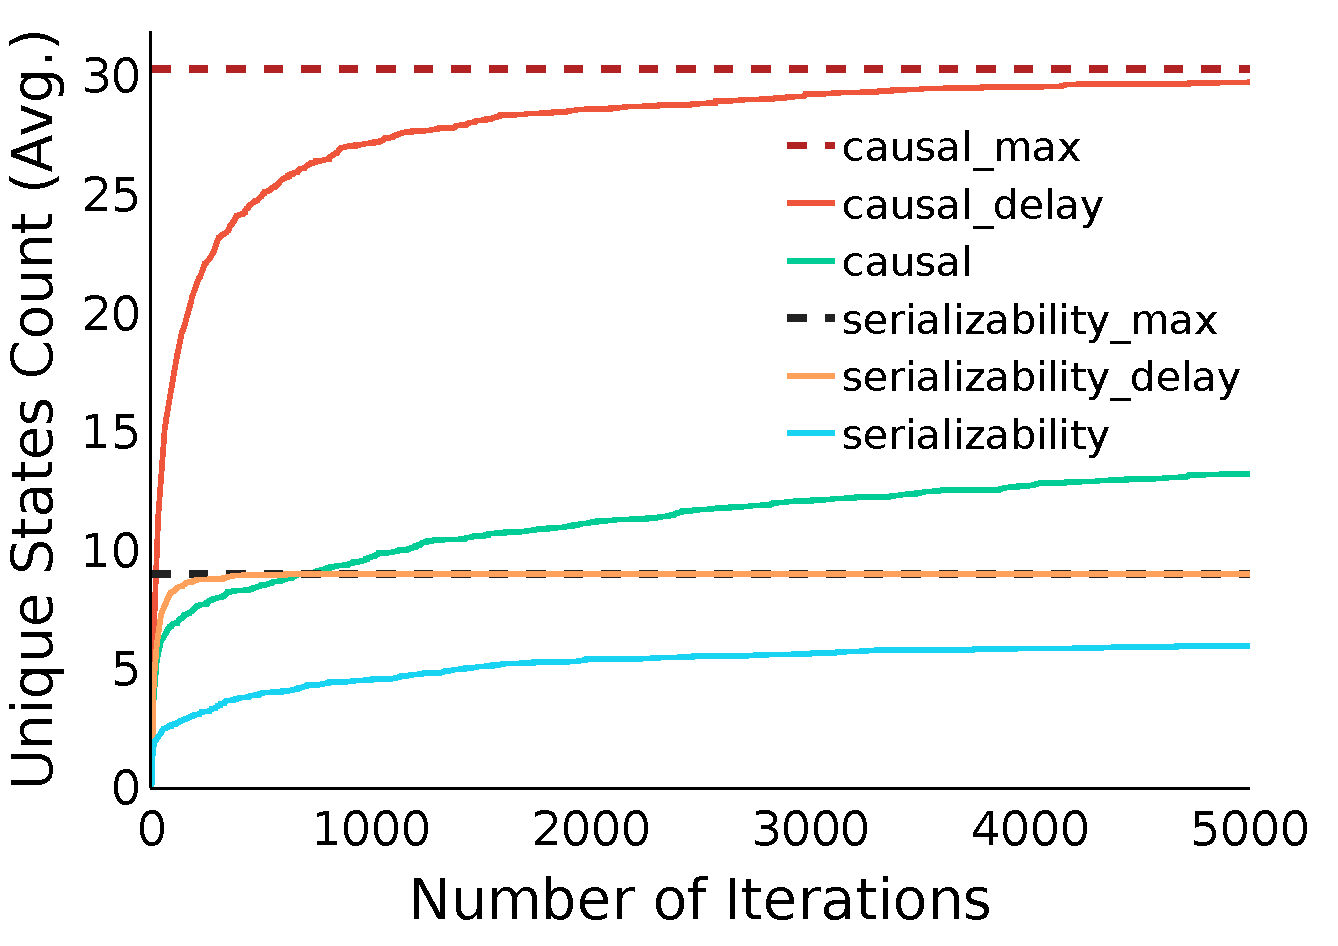
\includegraphics[width=0.4\textwidth]{plots/shopping_cart_random_avg.pdf}
%	
%	\caption{Shopping cart complete state exploration}
%	
%	\label{fig:cart_dfs}
%\end{figure}
%
%\begin{figure}[h]
%	
%	\centering
%	
%	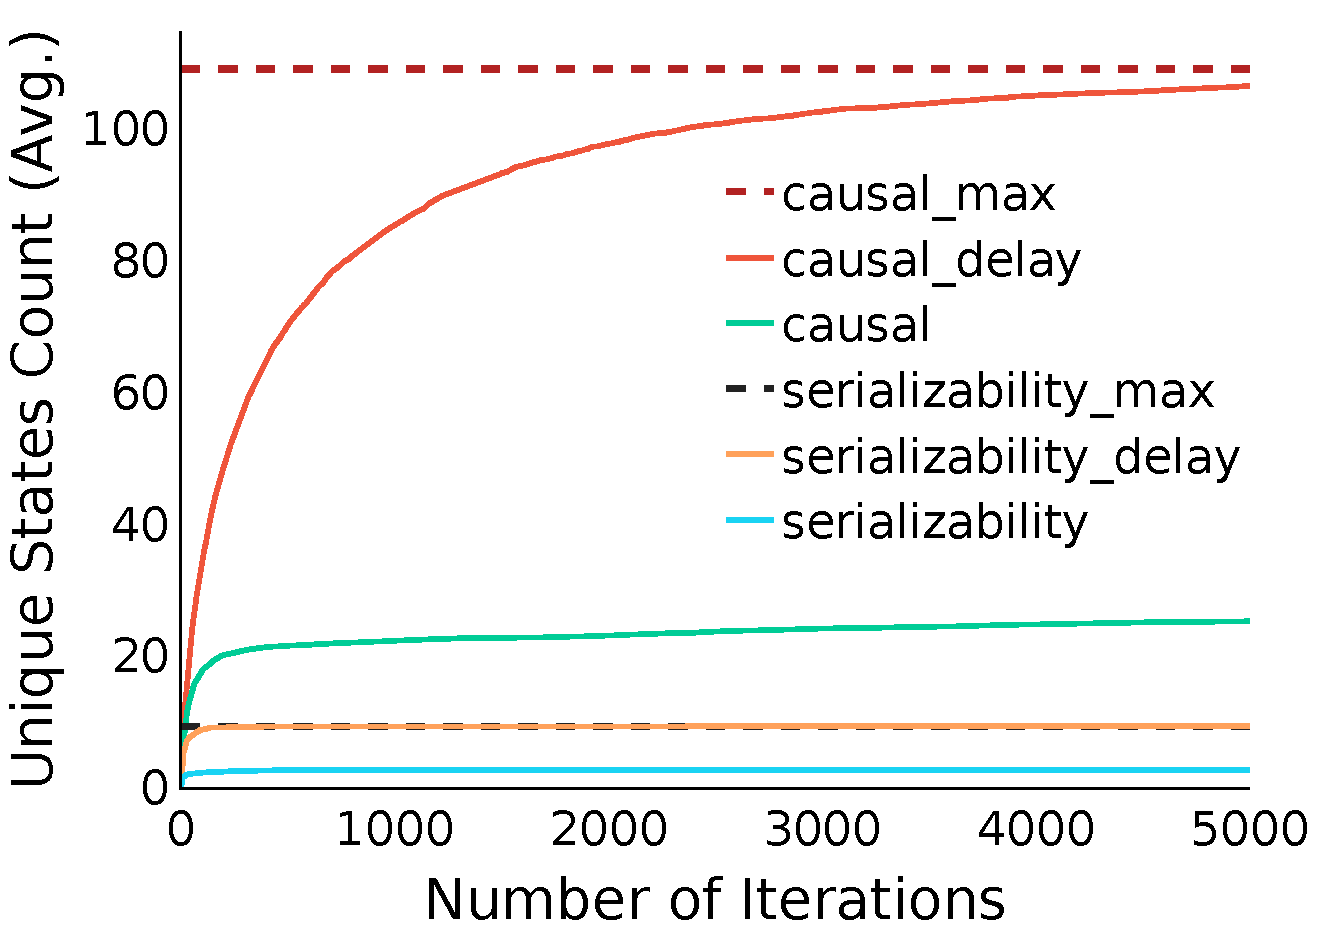
\includegraphics[width=0.4\textwidth]{plots/twitter_random_avg.pdf}
%	
%	\caption{Twitter complete state exploration}
%	
%	\label{fig:twitter_dfs}
%\end{figure}


%In the previous experiment, we were limited by DFS to explore all possible
%states, as it takes time to finish even for smaller test cases. We now show the
%effect of increasing the size of test case on the number of unique states
%observed. Figure \ref{fig:states_ops} shows the plot for stack application. We
%run stack application for 10,000 iterations with 3 threads and vary the number
%of operations per thread from 2 to 5. The states increase exponentially in
%causal consistency, but as we go towards larger test case, states tend to reach
%the upper limit possible to explore within 10,000 iterations.

%\begin{figure}[h]
%	
%	\centering
%	
%	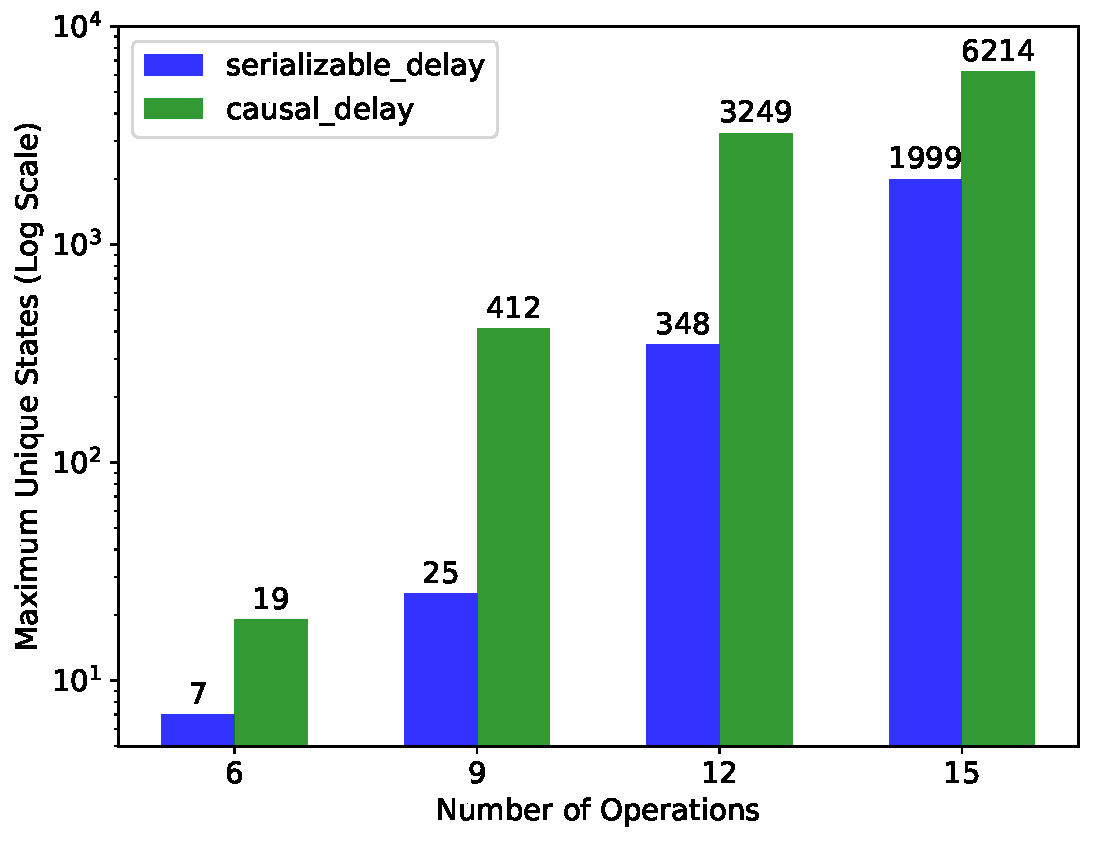
\includegraphics[width=0.5\textwidth]{plots/stack_states_op.pdf}
%	
%	\caption{Stack - maximum states possible with different operations}
%	
%	\label{fig:states_ops}
%\end{figure}
